\chapter{Introduction to Optics}
\label{chpt:optics}

\newthought{We introduce fundamental} concepts in optics by constructing a simplified model of a microscope.

Our model consists of two components: 1) a single lens and 2) an imaging plane (Figure \ref{fig:lens-equation}).
The lens\footnote{The lens is assumed to be a planar object.} can be thought of as a function that takes each ray of light emanating from a point on an object in the object plane and redirects them such that they fall on a corresponding point in the imaging plane.\footnote{The imaging plane corresponds to the face of a detector on a camera.}

\begin{figure}[h!!!]
    \centering
    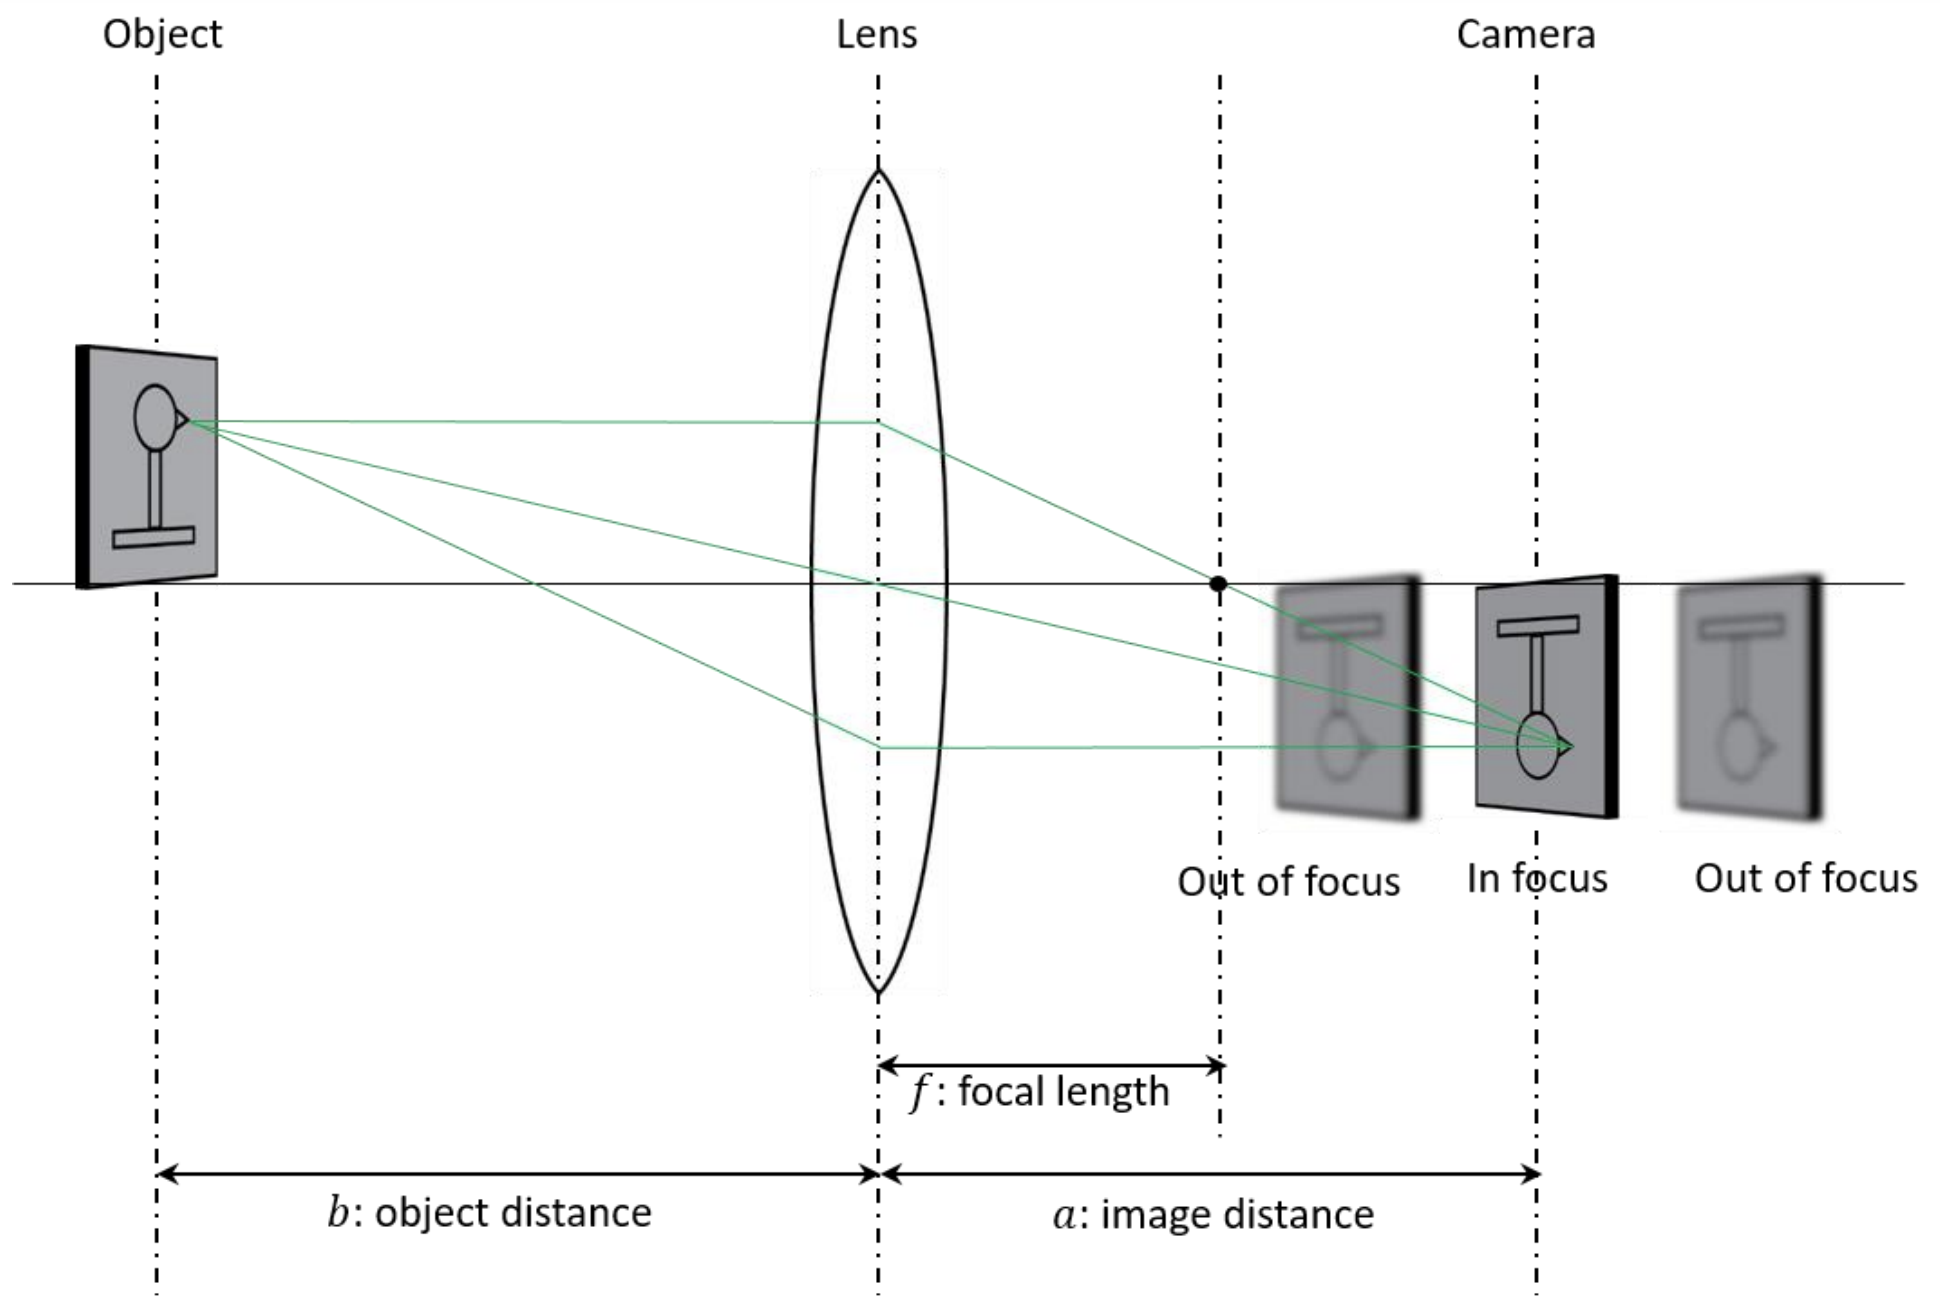
\includegraphics[width=\linewidth]{figs/lens-equation.png}
    \caption{A simplified model of an microscope imaging system with a single lens. Multiple rays of light emanate from a single source point on the object.}
    \label{fig:lens-equation}
\end{figure}

\begin{defn}[In-focus]
An image is \textbf{in-focus} if, for every source point on the object, all the emanating rays of light converge to a single point in the imaging plane.
\end{defn}

Therefore, to \textit{focus an image}, the object plane and image plane must be placed relative to the lens such that all rays of light converge.
This distance is governed by the \textbf{Lens Equation:}
\begin{equation}
    \label{eqn:lens}
    \frac{1}{b} + \frac{1}{a} = \frac{1}{f} \,,
\end{equation}
where $b$ is the distance from the object plane to the lens, $a$ is the distance from the lens to the image plane, and $f$ is the \textbf{focal length}.\footnote{The focal length, an intrinsic property of each lens, is the point at which parallel rays of light will converge.}
Therefore, if we know the focal length $f$ and either $a$ or $b$, we can compute the other distance.

For most lenses, there is a range of distances over which an object can appear\footnote{That is, as far as the human eye can perceive.} in-focus.
An aperture\footnote{A device that can narrow the beam of light exiting the lens} is a device that can also affect this sensitivity (Figure \ref{fig:aperture}).
The aperture places an upper bound on the maximum angle of rays that reach the image plane. 
The depth-of-focus\footnote{The range of distance over which an image appears in-focus.} of an imaging system is dependent on aperture size.
\begin{figure}
    \centering
    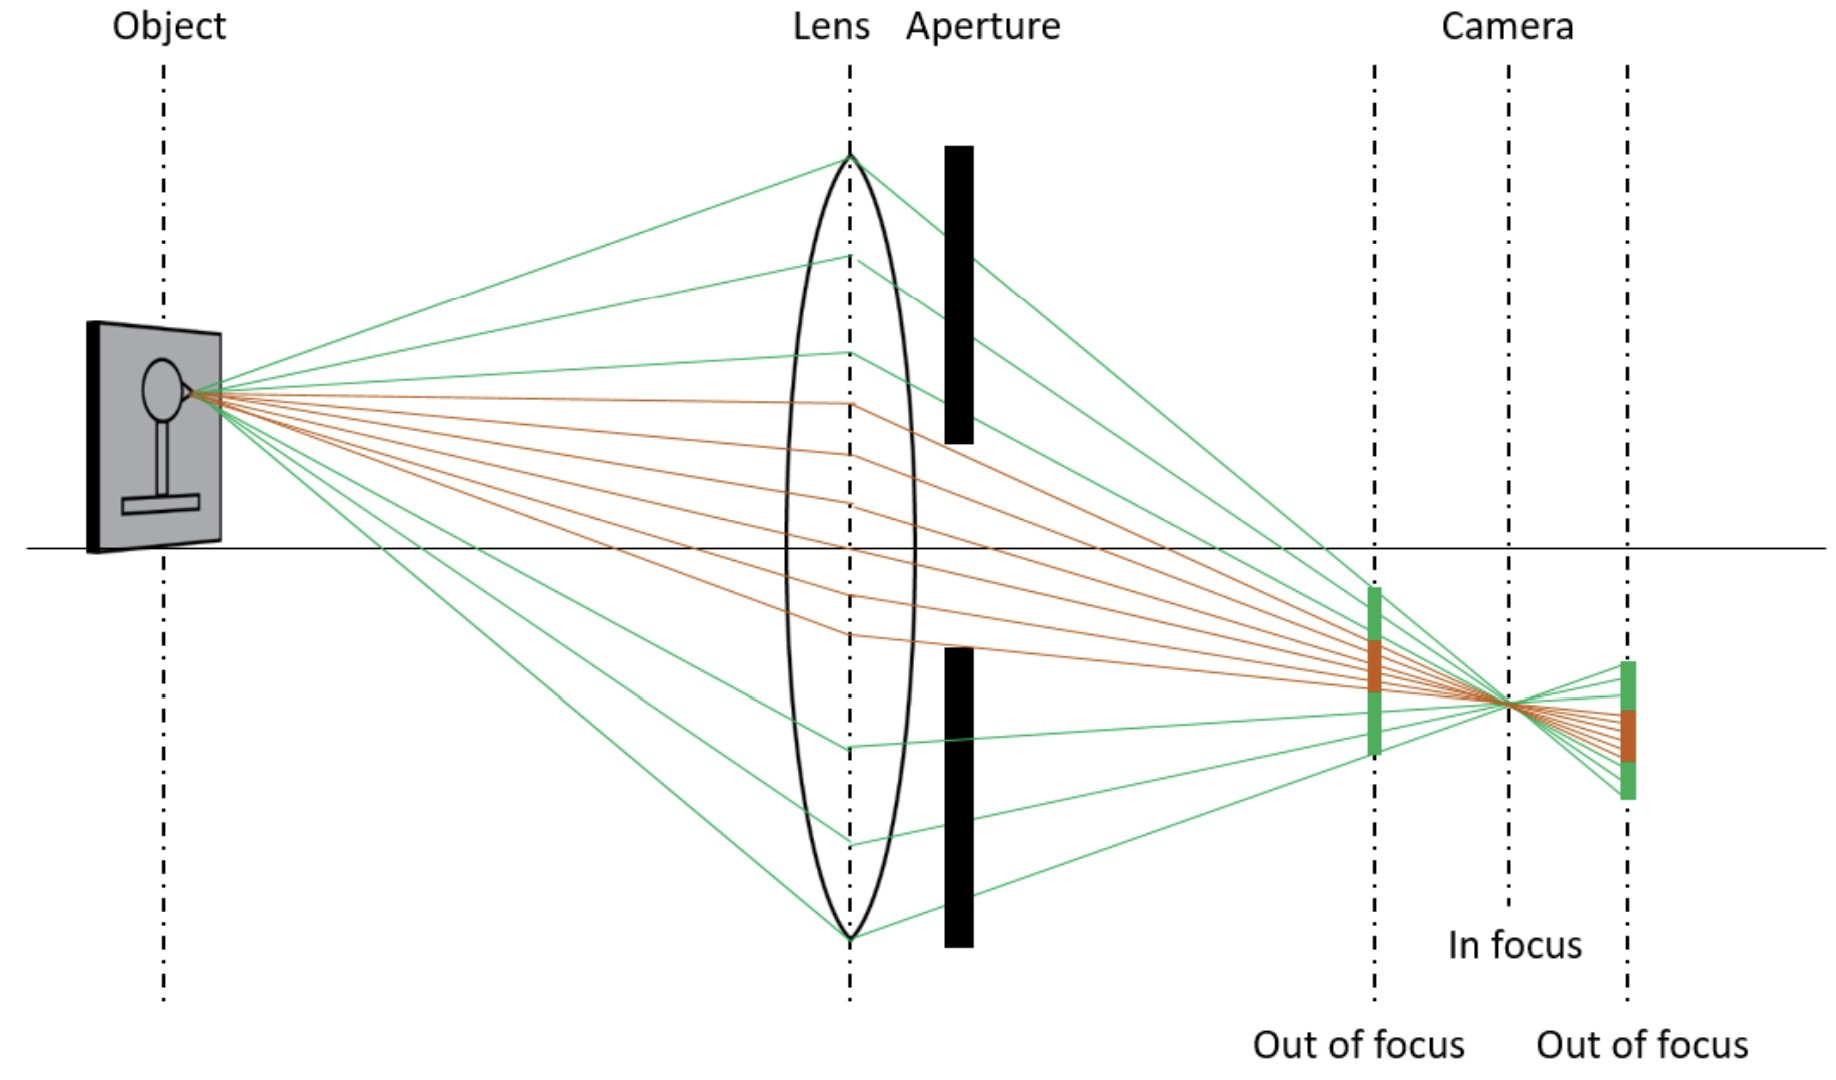
\includegraphics[width=\linewidth]{figs/aperture.png}
    \caption{An aperture occludes light that exits the lens. As we narrow the aperture, the upper bound on the angle of rays that are allowed to reach the image plane decreases. This reduces the numbers of rays from a source point that do not converge, creating \textit{less blur} in the image.}
    \label{fig:aperture}
\end{figure}

The final fundamental concept is \textbf{magnification} (Figure \ref{fig:magnification}). Magnification is the relative size of the image to the object: $M = \frac{a}{b} \,.$
\begin{figure*}
    \centering
    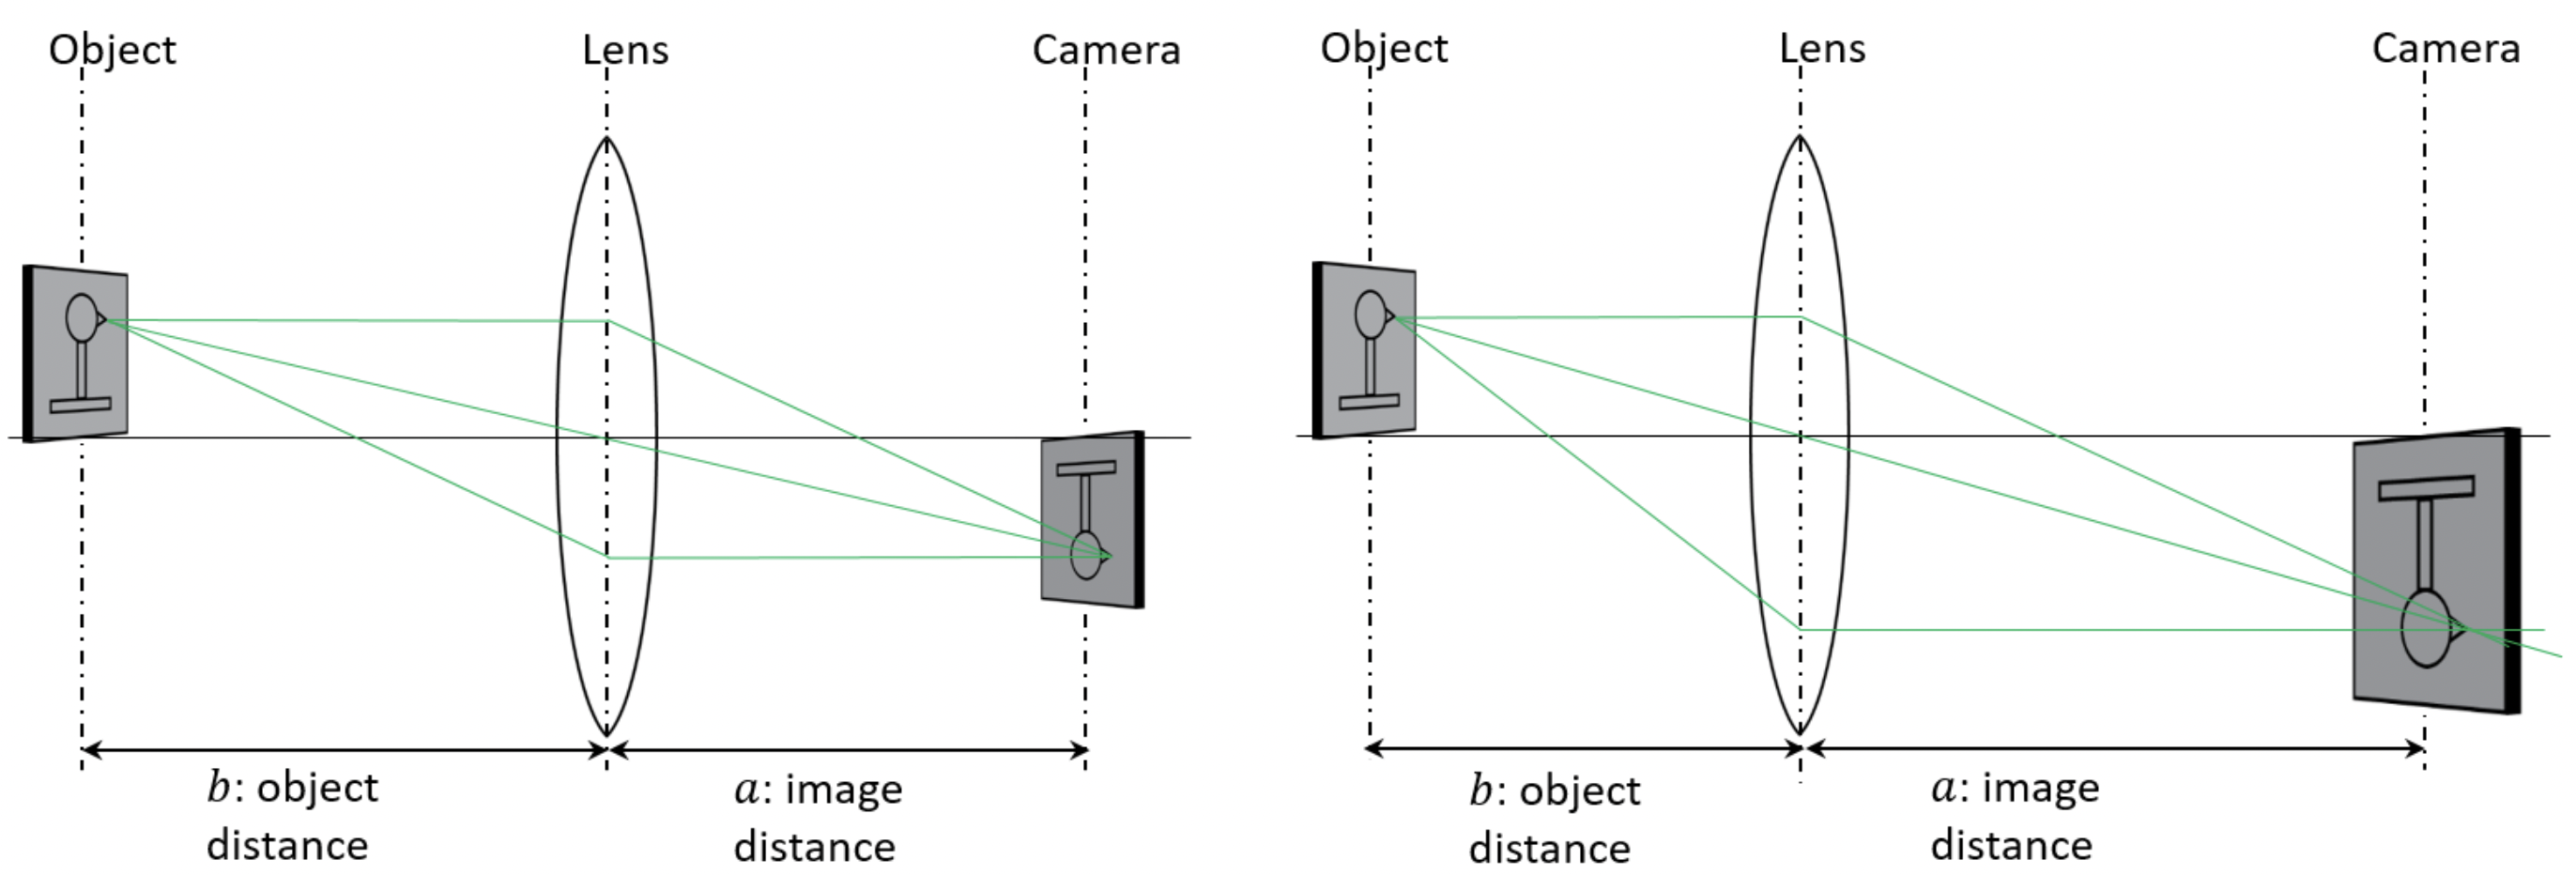
\includegraphics[width=0.95\linewidth]{figs/magnification.png}
    \caption{Magnification depends on the location of the lens relative to the object and imaging planes.}
    \label{fig:magnification}
\end{figure*}

\begin{question}
Suppose we measure magnification of two in-focus imaging systems by changing the distance from the camera by a known amount $z$ (see Figure \ref{fig:magnification} for the setup). 
Express the focal length $f$ in terms of these measurements.
\end{question}
\begin{answer}
Let $M_1 = \frac{a_1}{b_1}$ and $M_2 = \frac{a_1 + z}{b_2}$ be the two measured magnifications.
Because both systems are in-focus, the Lens Equation still holds:
\begin{align*}
    \frac{1}{f} &= \frac{1}{a_1} + \frac{1}{b_1} = \frac{a_1 + b_1}{a_1 b_1} = \frac{M_1 + 1}{a_1} \\
    \frac{1}{f} &= \frac{1}{a_1 + z} + \frac{1}{b_2} = \frac{a_1 + z + b_2}{(a_1 + z)b_2} = \frac{M_2 + 1}{a_1 + z}
\end{align*}
If we solve both equations for $a_1$, we get
\begin{align*}
    a_1 &= f(M_1 + 1) \\
    a_1 &= f(M_2 + 1) - z
\end{align*}
which yields
\begin{equation*}
    f = \frac{z}{M_2 - M_1} \,.
\end{equation*}
\end{answer}
